\doublespacing % Do not change - required

\chapter{Implementation}
\label{ch:implementation}

%%%%%%%%%%%%%%%%%%%%%%%%%%%%%%%%%%%%%%%
% IMPORTANT
\begin{spacing}{1} %THESE FOUR
\minitoc % LINES MUST APPEAR IN
\end{spacing} % EVERY
\thesisspacing % CHAPTER
% COPY THEM IN ANY NEW CHAPTER
%%%%%%%%%%%%%%%%%%%%%%%%%%%%%%%%%%%%%%%

This chapter documents the system as built, in the order the data flows through it. Section~\ref{sec:data_collection_pi} describes the paired-capture rig and the data collection, Section~\ref{sec:alignment_pipeline} the pipeline intended to produce aligned training pairs, and Appendix~\ref{app:ethics} the ethical and privacy considerations. Section~\ref{sec:nafnet_teacher} then details the NAFNet teacher, its block structure, training objective and convergence, and Section~\ref{sec:edge_deployment} the distillation, export and quantisation that produce the deployment-target student. The design rationale behind these choices is given in Chapter~\ref{ch:design}, and the numbers they produce are reported in Chapter~\ref{ch:results}.

\section{Data Collection}
\label{sec:data_collection_pi}

Supervised NIR$\rightarrow$RGB translation requires a paired dataset in which each NIR frame corresponds, pixel for pixel, to a visible RGB frame of the same image. No public dataset met this requirement (Section~\ref{sec:datasets}), so a bespoke capture rig was built and used to collect a large, urban dataset of London's streets.

\subsection{Capture rig}
\label{sec:hardware_setup}

The rig is a self-contained unit housed in a 3D-printed case (Figure~\ref{fig:capture_rig}). It contains a Raspberry Pi~5 and two Raspberry Pi Camera Module~3 sensors: one captures the visible RGB image, the other captures NIR through an 850\,nm IR long-pass filter that blocks visible light. To give both cameras the same optical perspective incoming light passes through a beam-splitter cube that divides it between the two sensors, so both image the scene through a shared aperture.

\begin{figure}[!htbp]
    \centering
    \begin{minipage}{0.62\textwidth}
        \centering
        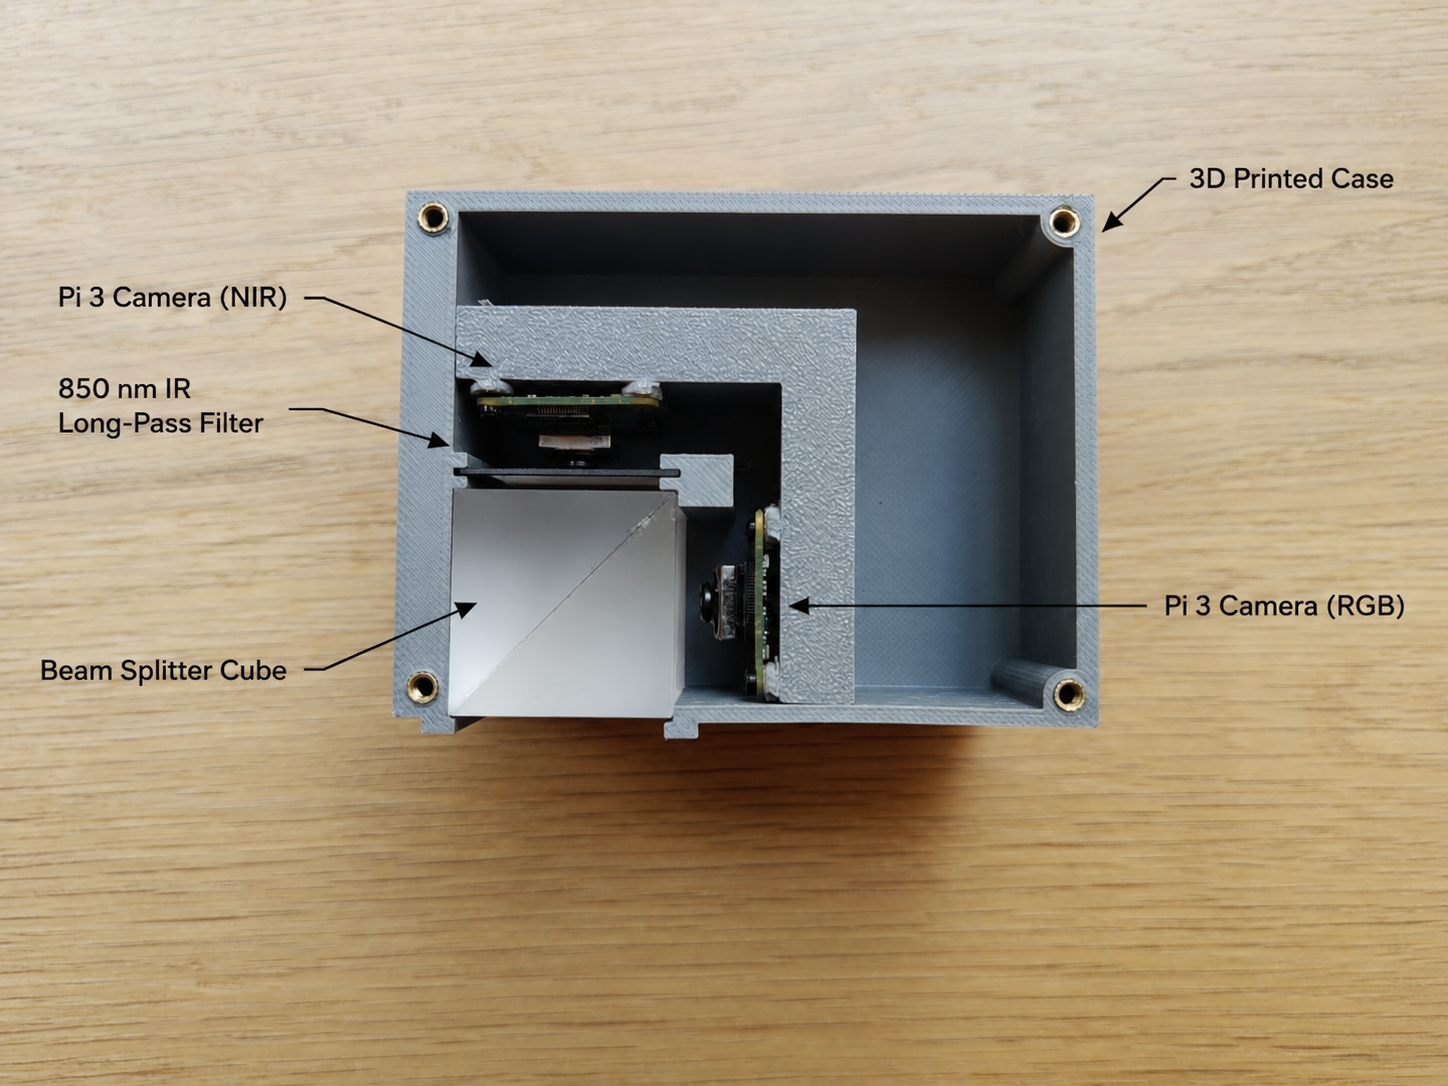
\includegraphics[width=\linewidth]{imgs/device-labeled.png}
        \subcap{(a) Internal layout (lid removed)}
    \end{minipage}
    \hfill
    \begin{minipage}{0.35\textwidth}
        \centering
        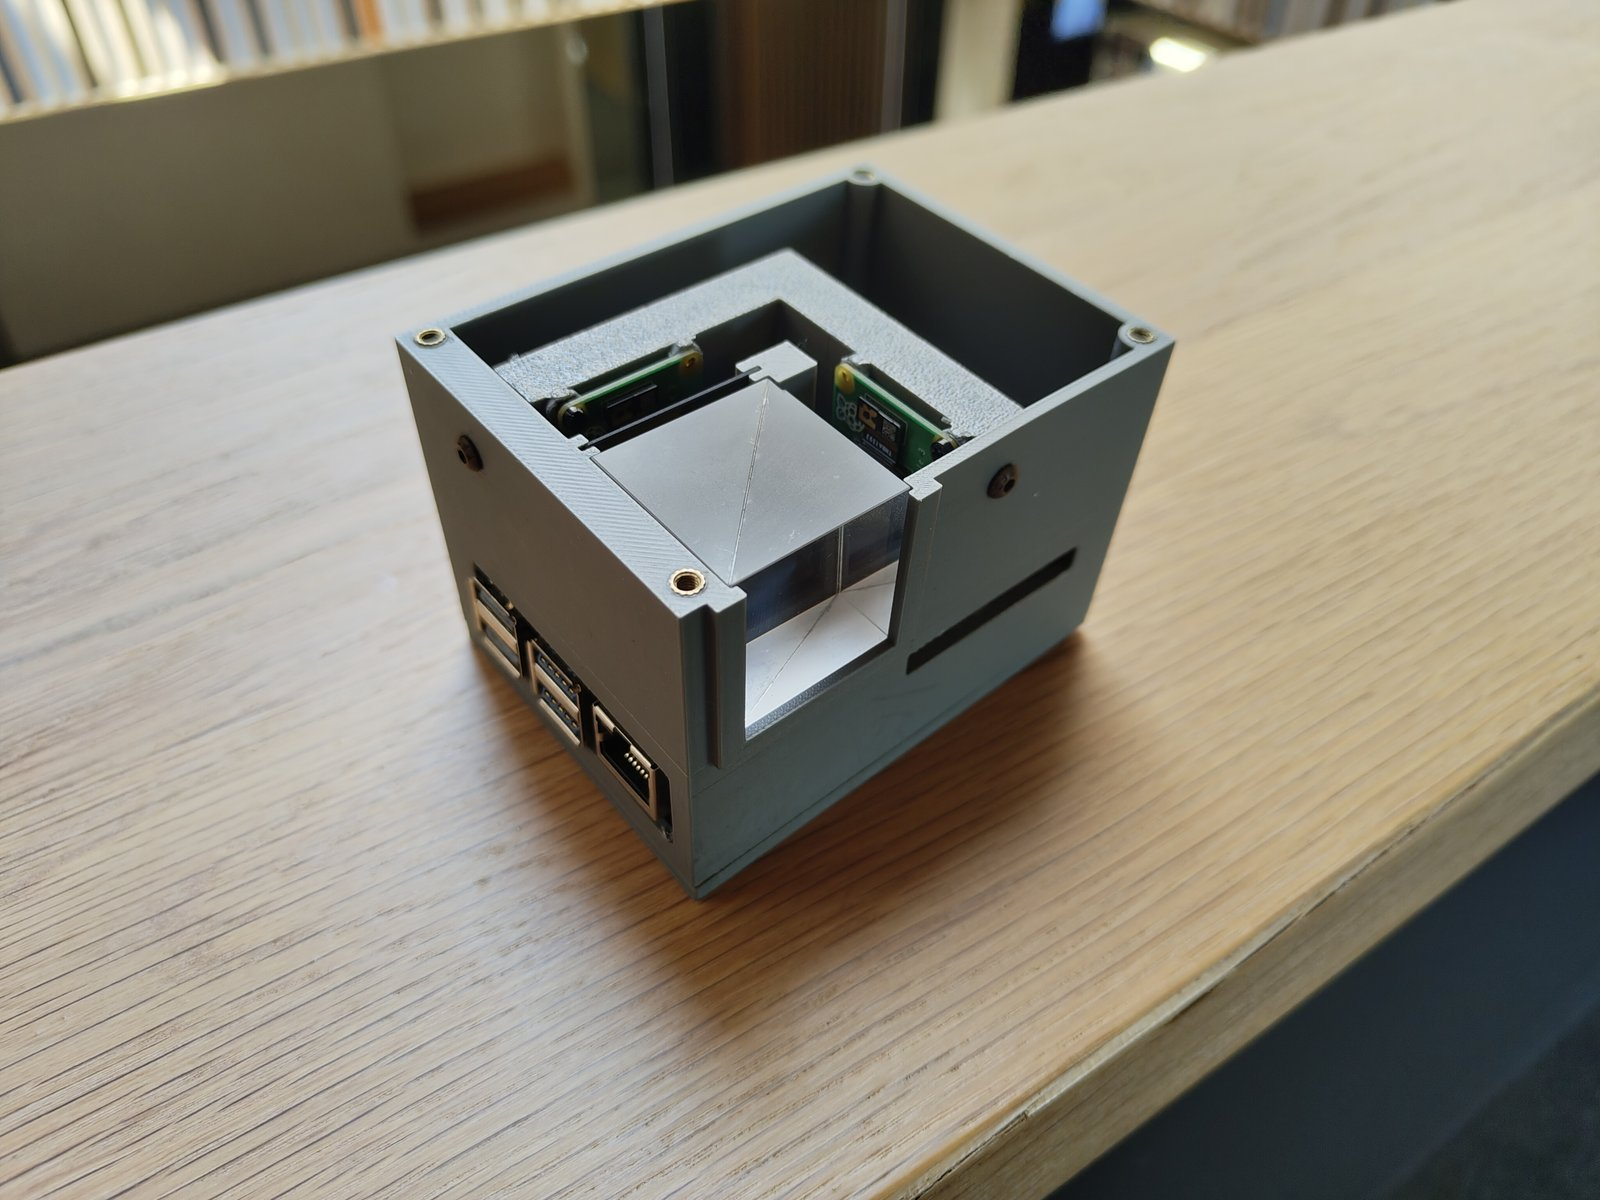
\includegraphics[width=\linewidth]{imgs/rig-internal-photo.jpg}
        \subcap{(b) Assembled rig (lid removed)}
    \end{minipage}
    \caption{The paired-capture rig. A beam-splitter cube feeds the same incoming light to a visible RGB camera and a NIR camera behind an 850\,nm long-pass filter.}
    \label{fig:capture_rig}
\end{figure}

The beam splitter gives both cameras a common optical centre, suppressing the depth-dependent parallax that no 2D warp could remove in a conventional side-by-side rig (Section~\ref{sec:intro_challenges}), at the cost of splitting the available light. With parallax suppressed, a single global homography can align the entire frame regardless of scene depth.

\subsection{Capture campaign}
\label{sec:capture_campaign}

Data was collected over more than 20 hours of cycling around London with the rig mounted on a backpack for hands-free capture (\autoref{fig:rig_deployed}), taking a paired NIR and RGB frame every 5 seconds. Cycling was chosen as it sweeps the rig continuously through diverse urban content. After the filtering and alignment pipeline described below \textbf{12{,}536} usable aligned pairs remained.

\begin{figure}[!htbp]
    \centering
    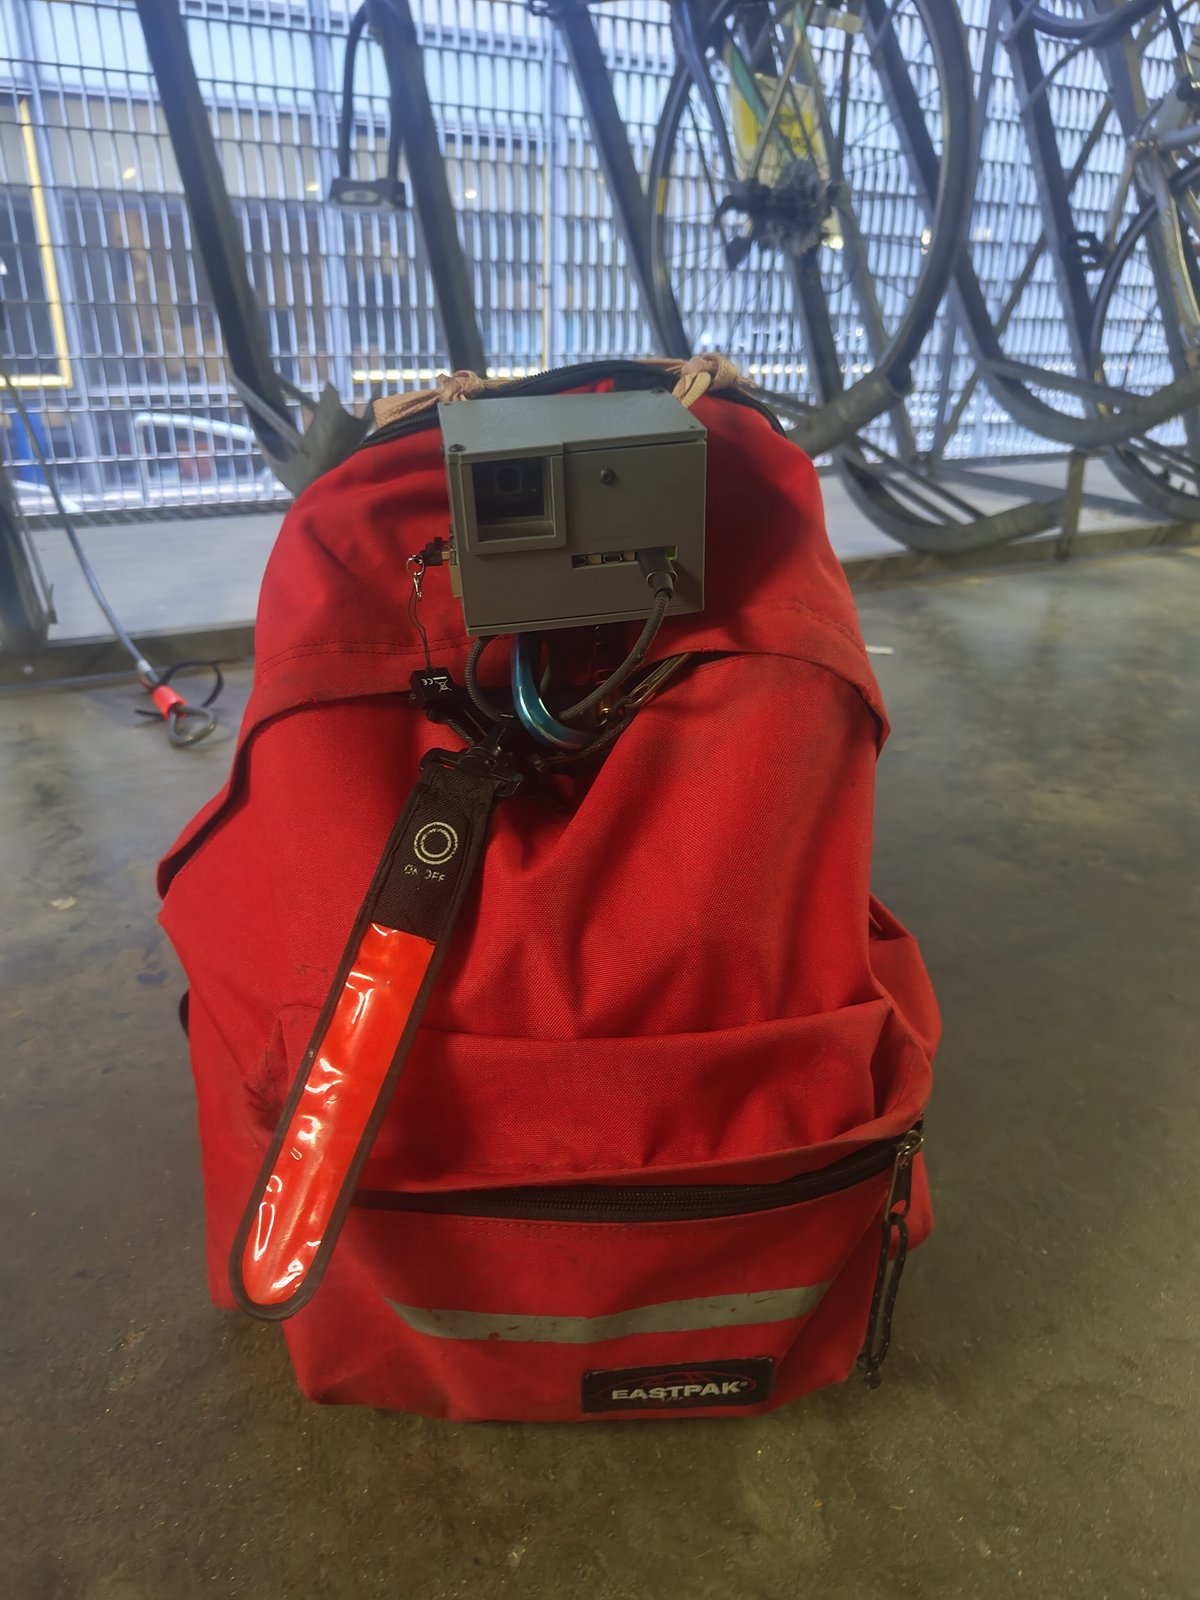
\includegraphics[width=0.5\textwidth]{imgs/rig-deployed.jpg}
    \caption{The capture rig mounted on a backpack for hands-free paired capture while cycling around London.}
    \label{fig:rig_deployed}
\end{figure}

\section{Producing Aligned Pairs}
\label{sec:alignment_pipeline}

Although the beam splitter suppresses parallax, the two optical paths are not pixel-identical. The cameras differ slightly in magnification, principal point and lens distortion, the IR filter shifts the focus of the NIR path, and the mounting can flex a little over a multi-hour ride. A per-pair alignment step absorbs these residual differences. Each raw capture starts as a full-frame RGB/NIR pair (\autoref{fig:pipe_pair}) and goes through the pipeline below. Figures~\ref{fig:pipe_pair}--\ref{fig:pipe_output} show the stages on one example capture.

\begin{figure}[!htbp]
    \centering
    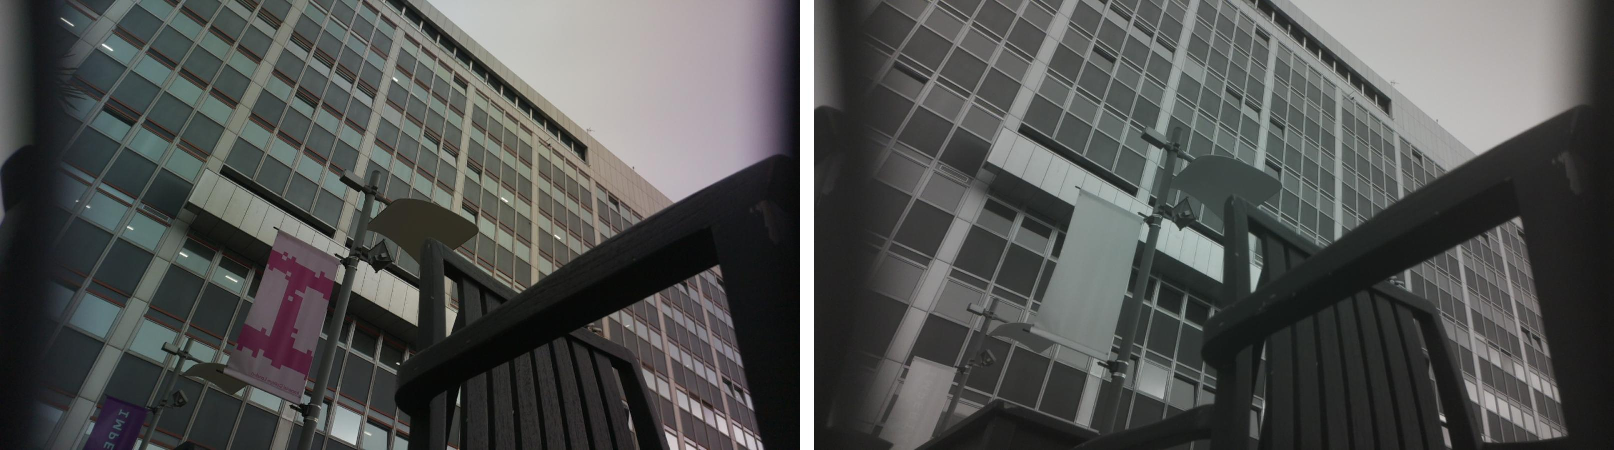
\includegraphics[width=0.9\linewidth]{imgs/pipeline_report/pipeline_01_pair.pdf}
    \caption{The raw captured pair before processing: the full-frame RGB (left) and NIR (right) straight from the two sensors. This is the input to the alignment pipeline.}
    \label{fig:pipe_pair}
\end{figure}

\paragraph{1.~Sharpness filtering.} Cycling introduces motion blur, which corrupts both the supervision target and the feature matching used for alignment. A sharpness score is computed as the variance of the Laplacian of a resized grayscale preview of the RGB frame. Pairs scoring below a threshold of 100 are rejected. The threshold was chosen by inspecting the Laplacian-variance distribution across a sample of captures, where it cleanly separates visibly sharp frames from motion-blurred ones. The example in Figure~\ref{fig:pipe_sharpness} scores 734.3 and is retained.

\begin{figure}[!htbp]
    \centering
    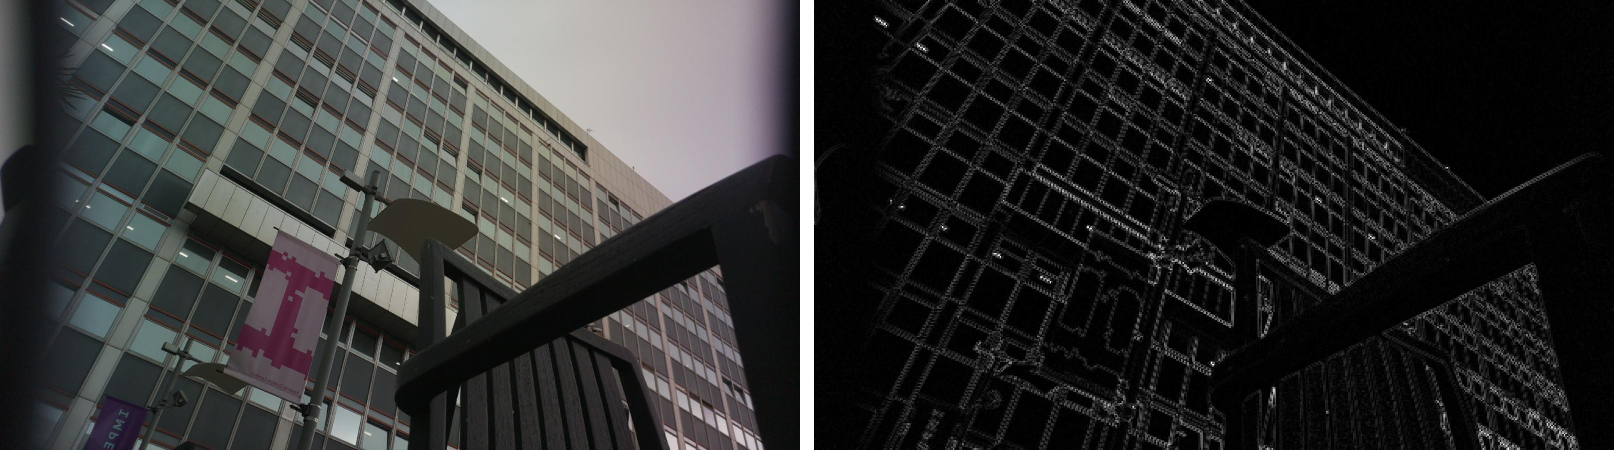
\includegraphics[width=0.9\linewidth]{imgs/pipeline_report/pipeline_02_sharpness.pdf}
    \caption{Sharpness assessment: the RGB frame and its Laplacian response. Frames whose Laplacian variance falls below the threshold (100) are discarded as too blurred for reliable supervision and feature matching.}
    \label{fig:pipe_sharpness}
\end{figure}

\paragraph{2.~Privacy and Anonymisation.} The rig was tilted upwards so pedestrians are not captured at close range, and the $256\times256$ output resolution removes identifying detail. The full privacy measures are set out in Appendix~\ref{app:ethics}.

\paragraph{3.~Square centre-crop.} Both frames are centre-cropped to a common square (\autoref{fig:pipe_crop}). This gives the two images an identical field of view and a consistent geometry for the feature detector.

\begin{figure}[!htbp]
    \centering
    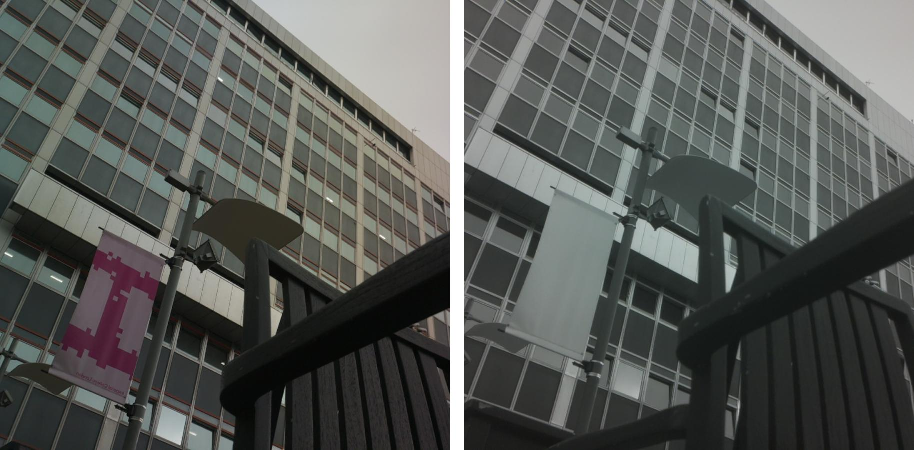
\includegraphics[width=0.7\linewidth]{imgs/pipeline_report/pipeline_03_crop.pdf}
    \caption{Square centre-crop of the RGB (left) and NIR (right) frames to a common field of view.}
    \label{fig:pipe_crop}
\end{figure}

\paragraph{4.~Feature-based alignment.} SIFT keypoints are detected in both crops and matched using Lowe's ratio test. RANSAC then estimates a homography that maps the NIR image onto the RGB image grid, rejecting inconsistent matches as outliers (Listing~\ref{lst:align}). SIFT was preferred over faster binary detectors such as ORB because alignment is a one-off offline step where match quality matters more than speed, and its scale- and rotation-invariant descriptors yield more inliers across the NIR/RGB appearance gap. For the example shown, 199 of 347 accepted SIFT matches are retained as homography inliers (Figure~\ref{fig:pipe_sift}).

\begin{lstlisting}[caption={Feature-based NIR$\rightarrow$RGB alignment: SIFT matching with Lowe's ratio test, followed by a RANSAC homography fit and warp.}, label={lst:align}]
kp_n, des_n = sift.detectAndCompute(nir, None)
kp_r, des_r = sift.detectAndCompute(rgb, None)
matches = matcher.knnMatch(des_n, des_r, k=2)
good = [m for m, n in matches if m.distance < 0.75 * n.distance]  # Lowe ratio
src = np.float32([kp_n[m.queryIdx].pt for m in good])
dst = np.float32([kp_r[m.trainIdx].pt for m in good])
H, inliers = cv2.findHomography(src, dst, cv2.RANSAC, 3.0)
nir_aligned = cv2.warpPerspective(nir, H, (width, height))
\end{lstlisting}

\begin{figure}[!htbp]
    \centering
    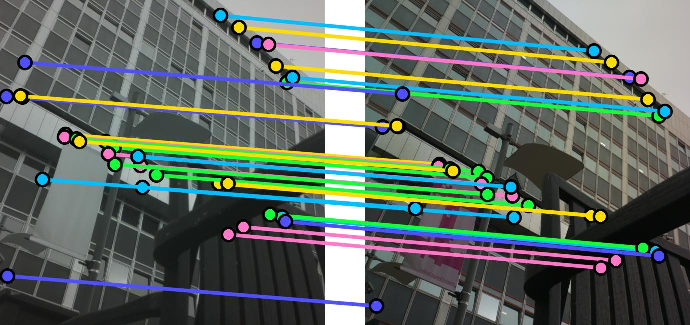
\includegraphics[width=0.9\linewidth]{imgs/pipeline_report/pipeline_04_sift.pdf}
    \caption{SIFT inlier correspondences (after Lowe's ratio test and RANSAC) used to estimate the NIR$\rightarrow$RGB homography for one capture: 199 inliers from 347 accepted matches.}
    \label{fig:pipe_sift}
\end{figure}

\paragraph{5.~Warp, overlap crop, resize, and export.} The NIR image is warped onto the RGB coordinate grid using the estimated homography. Both images are then cropped to their valid overlap region, centre-cropped to a common square, and resized to the $256\times256$ resolution used for storage and training. Captures that yield too few inliers, or a degenerate homography, are discarded at this stage. Figure~\ref{fig:pipe_output} shows a final homography-aligned pair.

\begin{figure}[!htbp]
    \centering
    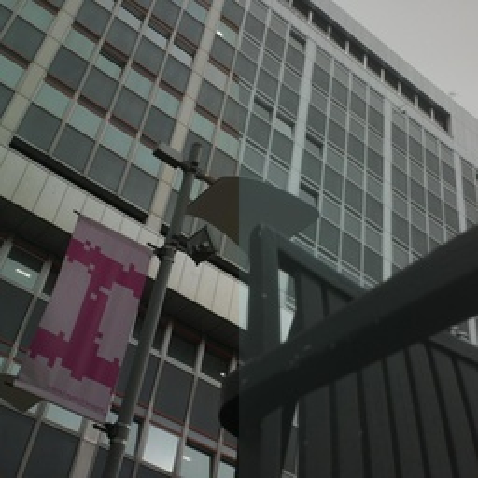
\includegraphics[width=0.9\linewidth]{imgs/pipeline_report/pipeline_05_output.pdf}
    \caption{Image pair, resized to the final $256\times256$ resolution and shown as a half-RGB (left), half-NIR (right) composite.}
    \label{fig:pipe_output}
\end{figure}

Applying this pipeline to the capture campaign produced the 12{,}536 retained pairs used for training and evaluation. The final protocol uses a fixed image-level 80/10/10 split, giving 10{,}028 training, 1{,}253 validation and 1{,}255 test pairs. 

\section{Translator Model: NAFNet Teacher}
\label{sec:nafnet_teacher}

The translator is NAFNet~\cite{chen2022nafnet}, a 2022 ``simple baselines'' architecture for image restoration, here configured for paired NIR$\rightarrow$RGB translation and trained as the high-quality \emph{teacher} for the project. It was chosen over a Pix2Pix-style U-Net for the reasons set out in Section~\ref{sec:architecture_choice}. This section documents the model as built. The reported configuration is the width-64 variant, with 116\,M parameters. \autoref{fig:nafnet_arch} shows the overall topology: a U-shaped encoder--bottleneck--decoder with additive skip connections, built entirely from the NAFBlock of \autoref{fig:nafblock}.

\begin{figure}[!htbp]
\centering
\begin{tikzpicture}[
  font=\scriptsize,
  stage/.style={rectangle, rounded corners, draw, fill=blue!8, minimum width=2.7cm, minimum height=0.95cm, align=center},
  mid/.style={rectangle, rounded corners, draw, fill=orange!18, minimum width=2.9cm, minimum height=0.95cm, align=center},
  io/.style={rectangle, rounded corners, draw, fill=gray!12, minimum width=2.4cm, minimum height=0.8cm, align=center},
  ar/.style={-{Latex[length=2mm]}, thick},
  sk/.style={-{Latex[length=2mm]}, dashed, gray!70!black}
]
\node[io]    (intro) at (0,1.15) {Intro conv\\$3\!\to\!64$};
\node[stage] (e1) at (0,0)      {Enc 1: $2\times$NAF\\$w{=}64$};
\node[stage] (e2) at (0,-1.25)  {Enc 2: $2\times$NAF\\$w{=}128$};
\node[stage] (e3) at (0,-2.5)   {Enc 3: $4\times$NAF\\$w{=}256$};
\node[stage] (e4) at (0,-3.75)  {Enc 4: $8\times$NAF\\$w{=}512$};
\node[mid]   (mid) at (3,-5.05)  {Bottleneck\\$12\times$NAF, $w{=}1024$};
\node[stage] (d1) at (6,-3.75)  {Dec 1: $2\times$NAF\\$w{=}512$};
\node[stage] (d2) at (6,-2.5)   {Dec 2: $2\times$NAF\\$w{=}256$};
\node[stage] (d3) at (6,-1.25)  {Dec 3: $2\times$NAF\\$w{=}128$};
\node[stage] (d4) at (6,0)      {Dec 4: $2\times$NAF\\$w{=}64$};
\node[io]    (end) at (6,1.15)  {Ending conv\\$64\!\to\!3$, \texttt{tanh}};
\draw[ar] (intro) -- (e1);
\draw[ar] (e1) -- (e2) node[midway,right]{$\downarrow2$};
\draw[ar] (e2) -- (e3) node[midway,right]{$\downarrow2$};
\draw[ar] (e3) -- (e4) node[midway,right]{$\downarrow2$};
\draw[ar] (e4) -- (mid) node[midway,below left]{$\downarrow2$};
\draw[ar] (mid) -- (d1) node[midway,below right]{PS$\uparrow2$};
\draw[ar] (d1) -- (d2) node[midway,left]{PS$\uparrow2$};
\draw[ar] (d2) -- (d3) node[midway,left]{PS$\uparrow2$};
\draw[ar] (d3) -- (d4) node[midway,left]{PS$\uparrow2$};
\draw[ar] (d4) -- (end);
\draw[sk] (e1.east) -- (d4.west) node[midway,above]{skip $\oplus$};
\draw[sk] (e2.east) -- (d3.west);
\draw[sk] (e3.east) -- (d2.west);
\draw[sk] (e4.east) -- (d1.west);
\end{tikzpicture}
\caption[NAFNet teacher architecture.]{The NAFNet teacher: a U-shaped encoder--bottleneck--decoder of NAFBlocks. Stride-2 convolutions downsample in the encoder, PixelShuffle (PS) upsamples in the decoder, and encoder features are \emph{added} ($\oplus$) into the matching decoder stage. The input is 3-channel NIR, the output 3-channel RGB in $[-1,1]$.}
\label{fig:nafnet_arch}
\end{figure}

\subsection{The NAFBlock}
\label{sec:nafnet_block_structure}

The network's only building block is the NAFBlock (\autoref{fig:nafblock}), and it contains \emph{no} conventional activation function. In place of a ReLU or GELU it uses a \emph{SimpleGate}: the feature map is split in half along the channel dimension and the two halves are multiplied elementwise.

\begin{lstlisting}[caption={The SimpleGate used in place of a nonlinear activation: the channels are split in half and multiplied elementwise.}, label={lst:simplegate}]
class SimpleGate(nn.Module):
    def forward(self, x):
        a, b = x.chunk(2, dim=1)   # split channels in half
        return a * b               # gate, no ReLU / GELU
\end{lstlisting}

Each block has two residual sub-blocks: a gated convolutional block (LayerNorm, $1{\times}1$ channel expansion, depthwise $3{\times}3$ convolution, SimpleGate, a lightweight squeeze-and-excitation channel reweighting, and a $1{\times}1$ projection) and a gated feed-forward block (LayerNorm, $1{\times}1$, SimpleGate, $1{\times}1$). Each sub-block is added back to its input through a learnable per-channel scale ($\beta$, $\gamma$) initialised to zero, so every block starts as an identity map and the deep stack trains stably from the first step.

The absence of nonlinear activations matters most for this project. With no saturating activations whose value distribution shifts under quantisation, the block keeps a predictable dynamic range, which eases the INT8 export discussed in Section~\ref{sec:edge_deployment}. It also leaves a small, standard operator set (convolution, layer normalisation, elementwise multiply and pixel shuffle) that exports cleanly to ONNX and the runtimes targeted for the edge device.

\begin{figure}[!htbp]
\centering
\begin{tikzpicture}[
  font=\scriptsize,
  op/.style={rectangle, rounded corners, draw, fill=blue!6, minimum width=3.4cm, minimum height=0.6cm, align=center},
  add/.style={circle, draw, inner sep=0.5pt, minimum size=0.5cm},
  ar/.style={-{Latex[length=1.6mm]}, thick}
]
\node            (in)  at (0,0)     {NAFBlock input};
\node[op]        (ln1) at (0,-0.8)  {LayerNorm};
\node[op]        (c1)  at (0,-1.6)  {$1{\times}1$ conv, $C\!\to\!2C$};
\node[op]        (dw)  at (0,-2.4)  {depthwise $3{\times}3$ conv};
\node[op]        (sg1) at (0,-3.2)  {SimpleGate ($2C\!\to\!C$)};
\node[op]        (sca) at (0,-4.0)  {$\times$ channel attention (SCA)};
\node[op]        (c3)  at (0,-4.8)  {$1{\times}1$ conv};
\node[add]       (a1)  at (0,-5.7)  {$+$};
\node[op]        (ln2) at (0,-6.6)  {LayerNorm};
\node[op]        (c4)  at (0,-7.4)  {$1{\times}1$ conv, $C\!\to\!2C$};
\node[op]        (sg2) at (0,-8.2)  {SimpleGate ($2C\!\to\!C$)};
\node[op]        (c5)  at (0,-9.0)  {$1{\times}1$ conv};
\node[add]       (a2)  at (0,-9.9)  {$+$};
\node            (out) at (0,-10.7) {NAFBlock output};
\draw[ar] (in)--(ln1); \draw[ar](ln1)--(c1); \draw[ar](c1)--(dw); \draw[ar](dw)--(sg1);
\draw[ar](sg1)--(sca); \draw[ar](sca)--(c3); \draw[ar](c3)--(a1);
\draw[ar](a1)--(ln2); \draw[ar](ln2)--(c4); \draw[ar](c4)--(sg2); \draw[ar](sg2)--(c5);
\draw[ar](c5)--(a2); \draw[ar](a2)--(out);
\draw[ar] (in.east) .. controls (3.4,0) and (3.4,-5.7) .. (a1.east) node[pos=0.5,right]{$\times\,\beta$};
\draw[ar] (a1.west) .. controls (-3.4,-5.7) and (-3.4,-9.9) .. (a2.west) node[pos=0.5,left]{$\times\,\gamma$};
\end{tikzpicture}
\caption{The NAFBlock: a gated convolutional sub-block followed by a gated feed-forward sub-block, with no nonlinear activation. The SimpleGate halves the channels and multiplies them. Learnable per-channel scales $\beta,\gamma$ (initialised to zero) gate each residual so the block starts as an identity map.}
\label{fig:nafblock}
\end{figure}

\subsection{Backbone configuration}
\label{sec:nafnet_backbone}

The encoder has four stages of [2, 2, 4, 8] NAFBlocks at channel widths [64, 128, 256, 512]; each stage is followed by a stride-2 $2{\times}2$ convolution that halves resolution and doubles the channel count. A bottleneck of 12 NAFBlocks runs at width 1024. The decoder mirrors the encoder with [2, 2, 2, 2] blocks, upsampling with PixelShuffle$\times$2. Encoder features are \emph{added} into the matching decoder stage rather than concatenated, which keeps channel counts, and therefore parameters, down. An intro $3{\times}3$ convolution lifts the 3-channel NIR input to width 64, and an ending $3{\times}3$ convolution maps back to 3 channels, followed by a \texttt{tanh} into $[-1,1]$. NAFNet's optional global input$\rightarrow$output residual is disabled, because NIR and RGB are different modalities and adding the input back would force the network to encode all colour as a delta on the NIR. \autoref{tab:teacher_config} summarises the configuration.

\begin{table}[!htbp]
\centering
\footnotesize
\begin{tabular}{ll}
\hline
\textbf{Component} & \textbf{Setting} \\
\hline
Generator & NAFNet, width 64 (116\,M params) \\
Encoder stages & $[2,2,4,8]$ blocks @ widths $[64,128,256,512]$ \\
Bottleneck & 12 blocks @ width 1024 \\
Decoder stages & $[2,2,2,2]$ blocks, PixelShuffle$\times2$ \\
Skip connections & additive (encoder $\to$ decoder) \\
Input / output & 3-ch NIR / 3-ch RGB, $256\times256$, \texttt{tanh}$\to[-1,1]$ \\
Global residual & disabled \\
Discriminator & $70\times70$ PatchGAN; GAN weight 0.3 (30-epoch warmup) \\
Feature-map ensemble & DINOv2/CLIP/ResNet-50 weights 40/20/5 (30-epoch warmup) \\
Optimiser & Adam; lr $2\times10^{-5}$; G $\beta(0.9,0.99)$, D $\beta(0.5,0.999)$ \\
Batch / precision & 1 / full precision (FP32), gradient clip 0.5 \\
Schedule & 200 epochs, trained from scratch (single stage) \\
Checkpoint selection & best validation CLIP cosine similarity \\
\hline
\end{tabular}
\caption{NAFNet teacher configuration for the run \texttt{ablation\_15b\_l1boost\_split42\_s2}. Epoch 199 was selected by the highest validation CLIP ViT-B/32 cosine similarity.}
\label{tab:teacher_config}
\end{table}

\subsection{Training objective}
\label{sec:teacher_loss}

The final teacher augments the conventional pixel-plus-adversarial recipe with a \emph{foundation-model feature-matching ensemble} (whose components are ablated individually in Chapter~\ref{ch:results}). Alongside an L1 colour term (weight 20), an MS-SSIM structural term (weight 3) and a lightly weighted adversarial PatchGAN term (weight 0.3, linearly warmed up over the first 30 epochs), most of the semantic supervision comes from matching the deep features of the prediction and the ground truth across three frozen pretrained backbones, namely DINOv2 ViT-S/14, CLIP ViT-B/32 and ResNet-50, each contributing a feature-space loss computed at $224\times224$. The feature-matching ensemble is also linearly warmed up over the first 30 epochs. Only the VGG-perceptual term is switched off (\autoref{tab:teacher_loss}). Unlike the multi-stage baseline, the teacher is trained from scratch in a single stage. The comparatively strong L1 anchor keeps the pixel-level signal competitive while the foundation-feature gradient is introduced, which stabilises single-stage convergence.

The rationale for replacing the single VGG perceptual term with this ensemble is set out in Section~\ref{sec:loss_design}. In keeping with that objective, checkpoints are selected on validation CLIP cosine similarity rather than PSNR.

\begin{table}[!htbp]
\centering
\footnotesize
\begin{tabular}{lcl}
\hline
\textbf{Loss term} & \textbf{Weight} & \textbf{Role} \\
\hline
L1 (pixel) & 20 & global colour anchor \\
MS-SSIM & 3 & structural similarity \\
Adversarial (LSGAN, $70\times70$ PatchGAN) & 0.3 & realism (30-epoch warmup) \\
DINOv2 ViT-S/14 feature match & 40 & semantic, self-supervised features \\
CLIP ViT-B/32 feature match & 20 & vision--language semantic features \\
ResNet-50 feature match & 5 & ImageNet convolutional features \\
VGG perceptual & 0 & disabled (used only by the baseline, Ch.~\ref{ch:results}) \\
\hline
\end{tabular}
\caption{The final teacher's training objective: L1 and MS-SSIM terms, a lightly weighted adversarial PatchGAN term, and a frozen foundation-model feature-matching ensemble. Each feature term is a feature-space loss computed at $224\times224$ on its backbone; the foundation-feature terms are linearly warmed up over the first 30 epochs.}
\label{tab:teacher_loss}
\end{table}

\subsection{Optimisation and convergence}
\label{sec:nafnet_training}

Training operates on $256\times256$ paired crops. NIR and RGB are augmented jointly with geometric transforms (random scale $[0.9,1.15]$, crop, horizontal flip, rotation up to $10^\circ$); the NIR input additionally receives photometric jitter (brightness $\pm0.2$, gamma $[0.8,1.2]$) so the translator is robust to the exposure variation that alignment cannot remove. Both tensors are normalised to $[-1,1]$.

Optimisation uses Adam (generator $\beta=(0.9,0.99)$, discriminator $\beta=(0.5,0.999)$) at a learning rate of $2\times10^{-5}$ in full precision; automatic mixed precision is disabled because the frozen foundation-model feature extractors were numerically more stable in FP32. Gradient clipping is set to 0.5 and the batch size to 1, which is memory-bound at $256^2$ with the 116\,M-parameter generator and three frozen feature extractors resident on the GPU. The adversarial and foundation-feature weights are ramped to their targets over the first 30 epochs. The teacher is trained from scratch in a single stage for 200 epochs. The translator is implemented in PyTorch, with version control via Git and experiment tracking through Weights \& Biases. Training was run mainly on Google Cloud \texttt{g2-standard-8} spot instances (NVIDIA L4), with up to four used in parallel for ablation sweeps, and on Imperial DoC workstations equipped with NVIDIA RTX~4080 (16\,GB), RTX~5090 (32\,GB) and RTX~6000 (48\,GB each). Checkpoints and training metrics are logged to Weights \& Biases for artefact retrieval and reproducibility.

\autoref{fig:training_curves} tracks the final teacher run. At the selected epoch 199 checkpoint, validation DINOv2-S cosine similarity is 0.9517, CLIP ViT-B/32 cosine similarity is 0.9090, PSNR is 26.497\,dB, SSIM is 0.8278 and LPIPS is 0.0985. PSNR is not the training target. The recipe trades a little pixel fidelity for stronger feature-space agreement, the quantity the downstream panel responds to. The checkpoint with the highest validation CLIP cosine similarity was selected for downstream evaluation. \autoref{fig:sample_grid} shows representative held-out test translations.

\begin{figure}[!htbp]
\centering
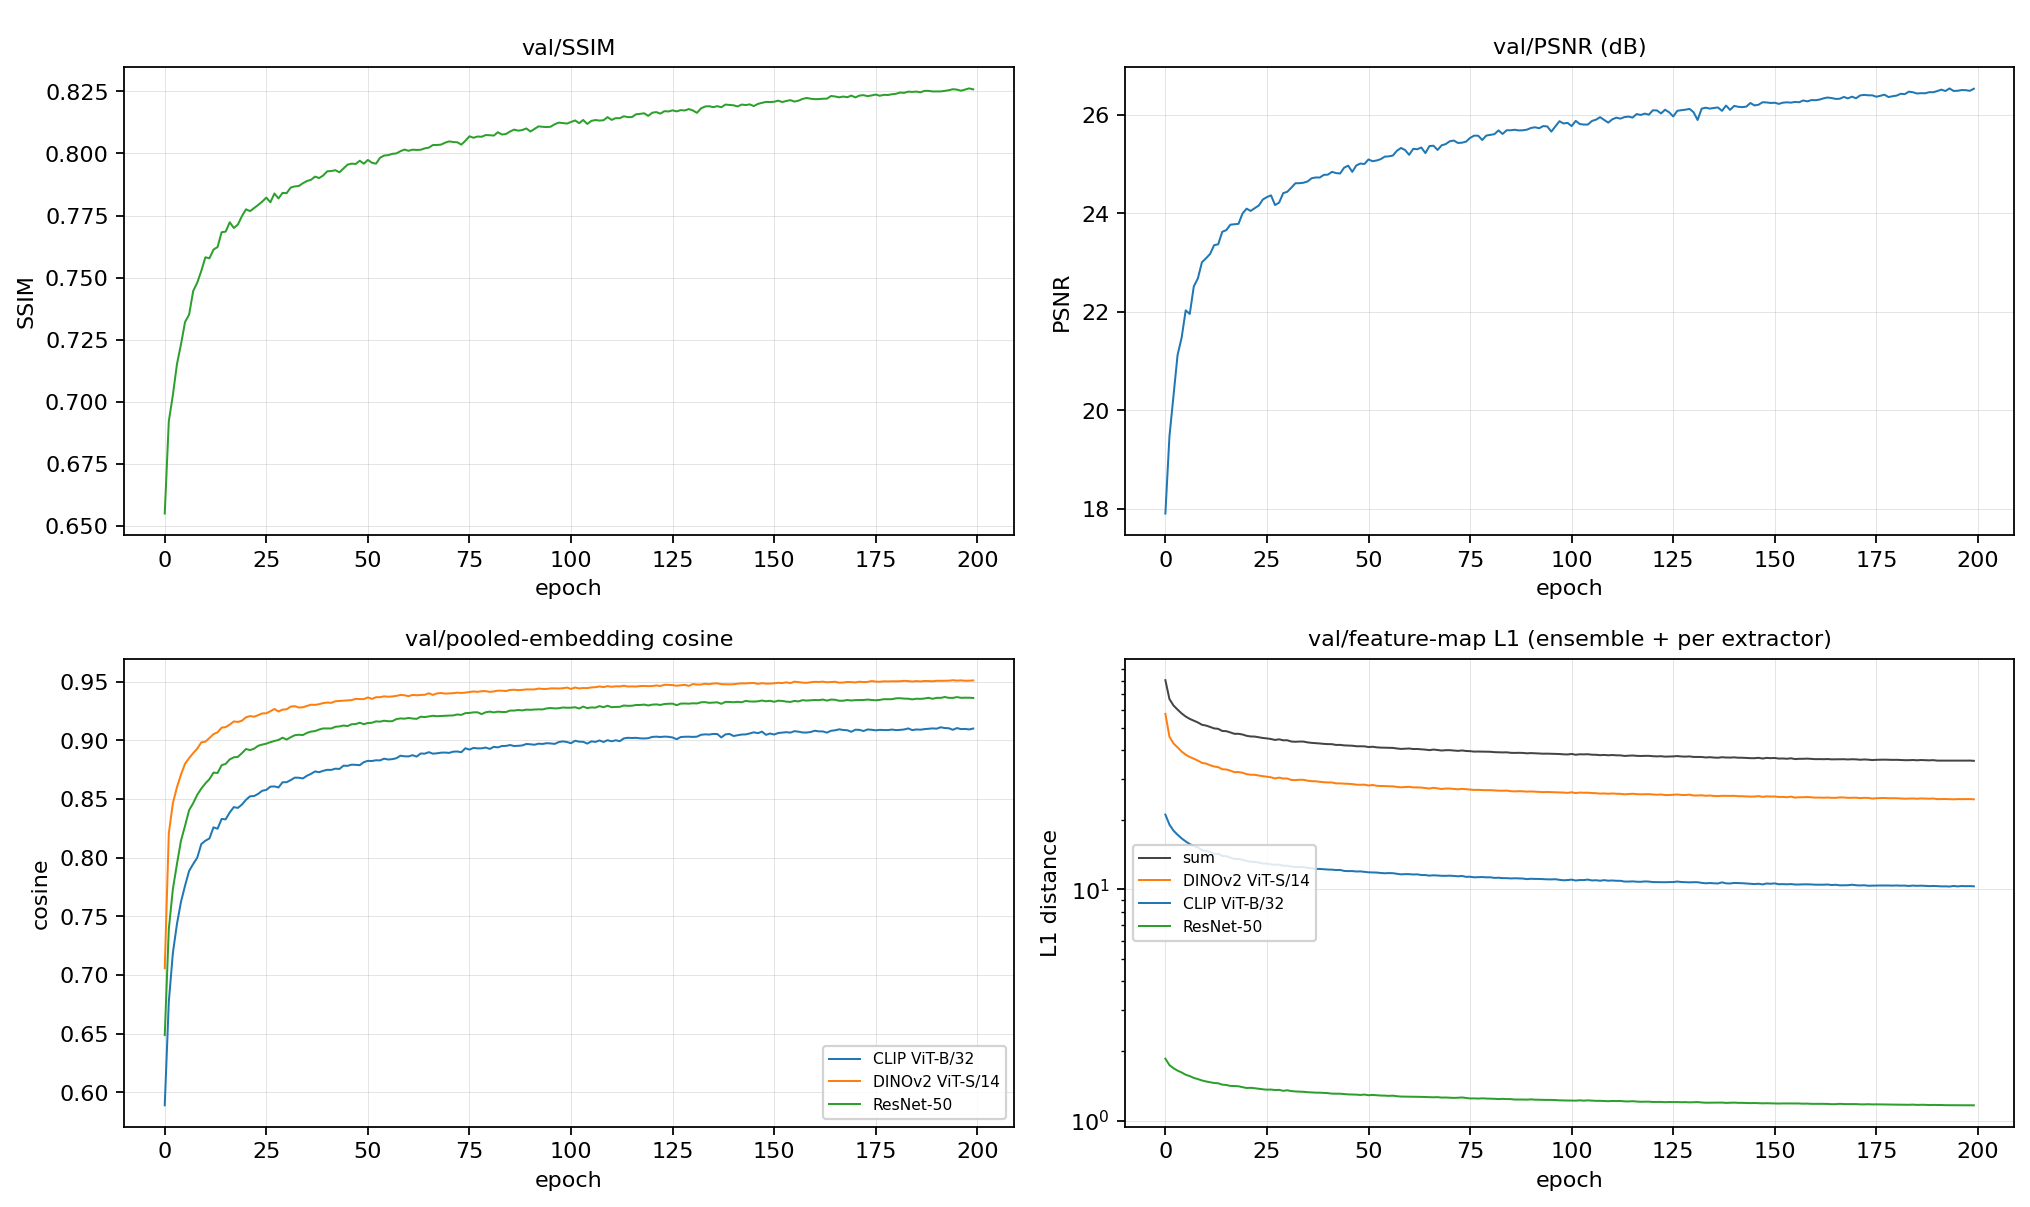
\includegraphics[width=\linewidth]{imgs/l1boost_curves.png}
\caption[Final-teacher validation metrics during training.]{Final-teacher validation metrics during training for \texttt{ablation\_15b\_l1boost\_split42\_s2} (foundation-ensemble objective; 200 epochs from scratch). Top left: SSIM and PSNR progress. Bottom left: pooled-embedding cosine similarity across three evaluators (CLIP ViT-B/32, DINOv2 ViT-S/14, ResNet-50). Bottom right: feature-map L1 distance showing alignment across extractors. Epoch 199 was selected by highest validation CLIP ViT-B/32 cosine similarity.}
\label{fig:training_curves}
\end{figure}

\begin{figure}[!htbp]
\centering
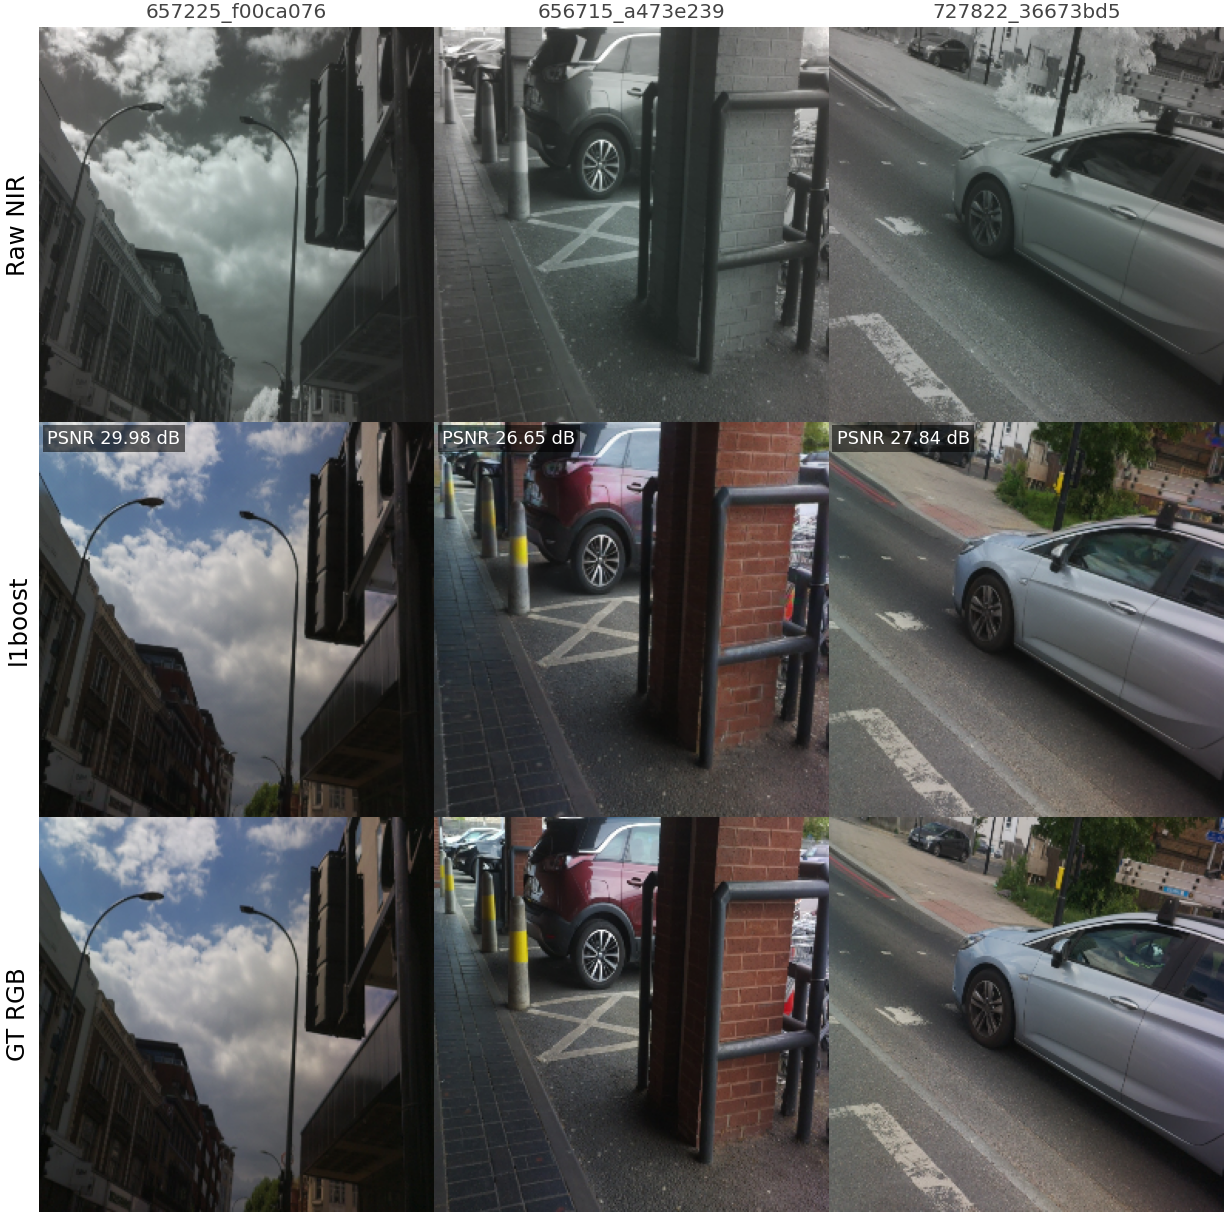
\includegraphics[width=\linewidth]{imgs/grid_22.png}
\caption{Five examples from the final foundation-ensemble teacher. The teacher recovers plausible colour and preserves scene structure across varied urban content.}
\label{fig:sample_grid}
\end{figure}

\section{Edge Deployment Path for the Raspberry Pi 5}
\label{sec:edge_deployment}

The teacher of Section~\ref{sec:nafnet_teacher} is not the intended deployment model; at 116\,M parameters it is too large for the Raspberry~Pi~5 target. The deployment path follows the teacher--student strategy of Section~\ref{sec:edge_student}: a compact student is distilled, exported and quantised to mixed INT8. The resulting artefact runs on the Pi~5 CPU, and a second export path targets the Hailo-8L neural accelerator on the Pi AI HAT+. Both are benchmarked on the device in Section~\ref{sec:impl_ondevice} and Section~\ref{sec:res_edge}.

\subsection{Distilled student}
\label{sec:impl_student}

A compact NAFNet is distilled from the width-64 teacher to target the Raspberry~Pi~5 CPU. It keeps the teacher's NAFNet block structure of the activation-free SimpleGate plus channel attention, so it inherits the same quantisation-friendly, export-clean operator set, and reduces only width and block depth. With width~16 and the shallowest depth (encoder blocks $[1,1,1,2]$, two middle blocks, decoder blocks $[1,1,1,1]$) it has only 1.7\,M parameters, roughly $1/67$ of the teacher, small enough for near-interactive inference on the CPU runtimes (Section~\ref{sec:impl_export}).

\begin{table}[!htbp]
\centering
\footnotesize
\begin{tabular}{lccc}
\hline
 & \textbf{CPU student} & \textbf{NPU student} & \textbf{Teacher} \\
 & \textbf{(width-16)} & \textbf{(width-32)} & \textbf{(width-64)} \\
\hline
Width          & 16          & 32          & 64          \\
Encoder blocks & $[1,1,1,2]$ & $[1,1,2,4]$ & $[2,2,4,8]$ \\
Middle blocks  & 2           & 4           & 12          \\
Decoder blocks & $[1,1,1,1]$ & $[1,1,1,1]$ & $[2,2,2,2]$ \\
Parameters     & 1.7\,M      & 11.6\,M     & 116\,M      \\
\hline
\end{tabular}
\caption{The distilled students against the teacher. Both students preserve the teacher's NAFNet block type and reduce only width and depth; the width-16 student is shaped for the Pi~5 CPU, and the larger width-32 variant for the Hailo-8L NPU (Section~\ref{sec:impl_hailo}).}
\label{tab:student_arch}
\end{table}

The student is trained to reproduce the teacher's outputs on the same data. The dominant term is a pixel-level distillation loss to the teacher's RGB output, with a smaller ground-truth L1 anchor and several frozen feature losses, optimising for downstream-representation fidelity rather than pixel mimicry alone (\autoref{tab:student_loss}). The teacher-output term is weighted more heavily than the ground-truth anchor to keep colour tied to measured RGB and limit amplification of teacher artefacts. The selected feature-KD student, \texttt{student\_l1b\_c\_featkd}, was selected at epoch 99 by validation CLIP cosine similarity 0.8585.
\pagebreak

\begin{table}[!htbp]
\centering
\footnotesize
\begin{tabular}{lcl}
\hline
\textbf{Loss term} & \textbf{Weight} & \textbf{Role} \\
\hline
Teacher-output L1 (distillation) & 50 & match the supervising teacher's RGB output \\
Ground-truth L1 & 5 & light colour anchor to real RGB \\
DINOv2 ViT-S/14 feature match & 40 & semantic, self-supervised features \\
CLIP ViT-B/32 feature match & 20 & vision--language semantic features \\
ResNet-50 feature match & 5 & ImageNet convolutional features \\
SegFormer-B0 ADE20K feature match & 15 & segmentation-sensitive features \\
DepthAnything-Small feature match & 10 & geometry-sensitive features \\
Teacher feature-KD match & 0.5 & match student and teacher feature representations \\
\hline
\end{tabular}
\caption{Training objective for the selected \texttt{student\_l1b\_c\_featkd} run. The teacher output is the dominant target, with a light ground-truth anchor, downstream-feature terms and an additional feature-KD term between student and teacher outputs.}
\label{tab:student_loss}
\end{table}

\begin{lstlisting}[caption={The student distillation objective: a dominant teacher-output L1 term, a light ground-truth anchor, and DINOv2/CLIP feature-matching terms.}, label={lst:distill}]
loss = (50.0 * l1(student_out, teacher_out)
        + 5.0 * l1(student_out, rgb_gt)
        + 40.0 * dinov2_feat(student_out, rgb_gt)
        + 20.0 * clip_feat(student_out, rgb_gt)
        + 5.0 * resnet_feat(student_out, rgb_gt)
        + 15.0 * segformer_feat(student_out, rgb_gt)
        + 10.0 * depth_feat(student_out, rgb_gt)
        + 0.5 * feature_kd(student_out, teacher_out))
\end{lstlisting}

\subsection{Export and quantisation}
\label{sec:impl_export}

All quantisation in this project is post-training, and no quantisation-aware training is used (Section~\ref{sec:quantisation}). A single FP32 PyTorch checkpoint is exported to the two runtimes representative of the Pi~5 software stack: ONNX Runtime, and LiteRT (formerly TFLite) executed through the XNNPACK CPU delegate. Export to ONNX uses opset 17 with a dynamic batch axis. Each runtime is benchmarked in full precision (FP32) and in INT8, with two ONNX INT8 variants compared: post-training static quantisation and a per-operator quantise/dequantise (Q/DQ) graph.

The calibration reader streams 100 representative NIR frames drawn deterministically from the seed-42 training split, preprocessed to the training range, and uses per-channel weight quantisation with MinMax activation ranges. With no saturating nonlinearities in the NAFBlock (Section~\ref{sec:nafnet_block_structure}), there is no activation clipping to calibrate around. A few structural operators still lack an INT8 kernel and are left in FP32, so the artefacts are a mixed INT8 rather than fully integer. In the ONNX path this is the PixelShuffle upsampling, which appears as a \texttt{DepthToSpace} node with no INT8 kernel at opset 17; the convolutions feeding it are excluded alongside it, so the optimiser does not strand them between quantise/dequantise pairs. In the LiteRT path the LayerNorm reductions remain in FP32 for the same reason.

The TFLite export was first produced with onnx2tf, but its NCHW$\rightarrow$NHWC layout pass mis-shaped the LayerNorm reduction tensors and broke the XNNPACK delegate. The export was therefore moved to Google's litert-torch, which lowers directly from the PyTorch graph and avoids the layout conversion entirely. The final LiteRT mixed-INT8 artefact is deterministic, occupies 2.3\,MB and retains positive gap closure on all five primary tasks. It executes through XNNPACK on the Pi's ARM CPU, and the measured runtime is reported in Section~\ref{sec:impl_ondevice}.

\subsection{Hailo-8L NPU export}
\label{sec:impl_hailo}

The Raspberry Pi AI HAT+ adds a Hailo-8L neural accelerator to the Pi~5, so a second export path was built to run the student on the NPU rather than the CPU. The Hailo toolchain does not accept the LiteRT or ONNX-Runtime artefacts directly. The FP32 ONNX student is recompiled to a Hailo Executable Format (HEF) file with the Hailo Dataflow Compiler 3.33.1 targeting the hailo8l architecture, which parses the graph, quantises it to INT8 from the same 100-frame calibration set, and allocates the network across the accelerator clusters.

Three operator issues had to be resolved before the graph would compile, and each was fixed without changing the network numerically. First, the PyTorch ONNX export omitted the explicit kernel shape on the convolutions, which the parser requires, so the attribute was restored from the weight tensors. Second, the NAFNet SimpleGate, a channel split followed by an element-wise multiply, is not a supported pattern, so it was rewritten as two $1\times1$ identity-selector convolutions feeding the same multiply, an exact reformulation. Third, the global average pooling in the channel-attention blocks could not be quantised directly because its reduction range was too large, so it was decomposed into a two-stage reduction. With these fixes both the width-16 student and the larger width-32 student variant (11.6\,M parameters; configuration in \autoref{tab:student_arch}) compiled cleanly, into HEF files of 17.7 and 50.4\,MB respectively, each taking a UINT8 $256\times256\times3$ input and producing a UINT8 output of the same shape. The cost of this path is its fragility: the surgery is specific to this operator set and compiler version, and the compiler ships only inside the vendor container rather than as a public package.

\subsection{On-device performance}
\label{sec:impl_ondevice}

The selected student was benchmarked on the Raspberry~Pi~5, on the CPU through LiteRT and on the Hailo-8L NPU. On the CPU the mixed-INT8 student runs at 5.05\,FPS measured at the model call, and on the NPU the same student runs at 27.2\,FPS with a 36.3\,ms hardware latency. Both backends meet the 5\,FPS target, the model footprint stays well inside the Pi's 8\,GB with no swap, and a sustained NPU run showed no thermal throttling. Section~\ref{sec:res_edge} reports the full figures and the requirement decisions.
